\section{Proceso de Desarrollo}

Proceso de desarollo integrado en la forja \textbf{SidelabCodeStack}.

\begin{itemize}
\item
  \href{001-git-introduccion.html}{Introducción}: \texttt{Git}
\item
  Visión general del \href{002-proceso-git.html}{proceso de desarrollo
  con \texttt{Git}}
\item
  Gestión de repositorios \href{003-gerrit-git.html}{\texttt{Git} con
  \texttt{Gerrit}}
\item
  Proceso de desarrollo con
  \href{003-eclipse.html}{\texttt{Eclipse IDE}}
\item
  \href{004-jenkins.html}{Integración continua} \texttt{Jenkins}
\end{itemize}
\section{Git}

\begin{figure}[htbp]
\centering

\includegraphics{images/git-logo.png}
\caption{}
\end{figure}

\textbf{Git} es un SCM distribuido (DSCM) en donde cada desarrollador
tiene una copia del repositorio.

No hay concepto de repositorio centralizado pero al final suele haberlo.

\subsection{Características}

\subsubsection{Snapshots}

En el repositorio \textbf{Git} no se guardan diferencias se guardan
snapshots en comparación con Subversion.

\begin{figure}[htbp]
\centering
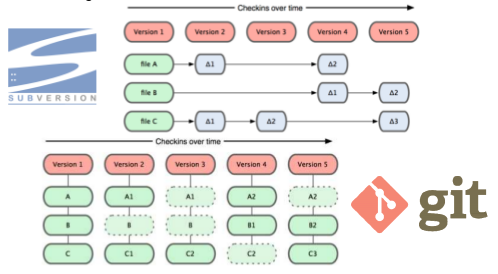
\includegraphics{images/svn-git-comparison.png}
\caption{}
\end{figure}

\subsubsection{Integridad}

Los commits se identifican por un \texttt{hash sha1}

\begin{itemize}
\item
  \texttt{Svn}: \emph{rev 33}
\item
  \texttt{Git}: \emph{d025a7b3217f05110ebbf48065b8d02a0ad22ae3}
\end{itemize}
O más amigablemente: \emph{d025a7b}

Los ficheros también se identifican por su sha1 de esta forma si un
fichero se corrompe durante la transmisión por la red se detecta
inmediatamente

\subsubsection{Los 3 estados}

Los ficheros en git pueden estar en tres estados:

\begin{itemize}
\item
  \texttt{Modificado}: el fichero ha cambiado desde el último checkout
\item
  \texttt{Staged}: un fichero modificado ha sido marcado para ser
  añadido en el próximo commit
\item
  \texttt{Committed}: el fichero se encuentra en la base de datos de git
\end{itemize}
Hay un 4º estado: \textbf{untracked}.

\subsubsection{Las 3 áreas de un proyecto git}

\begin{enumerate}
\item
  El directorio git (git directory):
  \begin{itemize}
  \item
    Contiene los metadatos y la base de datos de git
  \item
    Es lo que se copia cuando se clona un repositorio
  \item
    Normalmente es una carpeta .git en algún directorio
  \end{itemize}
\item
  La carpeta de trabajo (working directory):
  \begin{itemize}
  \item
    Es un checkout de una versión específica del proyecto
  \item
    Se extrae del directorio git
  \item
    Es el espacio donde modificamos los ficheros
  \end{itemize}
\item
  Staging area:
  \begin{itemize}
  \item
    Fichero en el directorio git que indica qué cambios van en el
    próximo commit
  \end{itemize}
\end{enumerate}
!(center)images/git--3-areas.png!

\subsubsection{La identidad}

Git necesita conocer algunos datos del desarrollador (aparecen en los
commits para identificar al autor)

\begin{itemize}
\item
  Nombre
\item
  Email
\end{itemize}
Si no están correctamente configurados pueden aparecer varios problemas:

\begin{itemize}
\item
  Los commits \textbf{fallan} porque el usuario no está autorizado
\item
  Commits del mismo usuario \emph{``físico''} \textbf{no son
  considerados como del mismo usuario} porque el nombre
  \emph{``lógico''} cambia.
\end{itemize}
Por lo que se ha de tener muy en cuenta este apartado y configurar
correctamente en el archivo \texttt{\ensuremath{\sim}}.

\begin{verbatim}
<code class="shell">$ patxi@patxi-PORTEGE-R830:~$ cat .gitconfig 
[user]
    name = patxigortazar
    email = patxi.gortazar@gmail.com
$ git config --global user.name “patxigortazar”
$ git config --global user.email “patxi.gortazar@gmail.com”
$ cd [path-to-gitrepo]
[path-to-gitrepo]$ git config user.name “patxigortazar”
[path-to-gitrepo]$ git config user.email “patxi.gortazar@gmail.com”
</code>
\end{verbatim}
\begin{quote}
\href{http://git-scm.com/book/en/Customizing-Git-Git-Configuration}{Follow~The~Yellow~Brick
Road}

\end{quote}
\paragraph{Comprobar la identidad}

Who am I?

\begin{verbatim}
<code class="shell">$ git config --list
user.name=patxigortazar
user.email=patxi.gortazar@gmail.com
</code>
\end{verbatim}
\subsubsection{Clientes git}

\begin{itemize}
\item
  En Eclipse
  \begin{itemize}
  \item
    Egit (viene por defecto en las últimas versiones)
  \end{itemize}
\item
  CLI Linux client
  \begin{itemize}
  \item
    sudo apt-get install git
  \end{itemize}
\item
  Windows
  \begin{itemize}
  \item
    Msysgit:
    \href{http://code.google.com/p/msysgit/downloads}{http://code.google.com/p/msysgit/downloads}/
  \item
    Tortoise Git (requiere msysgit):
    \href{http://code.google.com/p/tortoisegit/wiki/Download}{http://code.google.com/p/tortoisegit/wiki/Download}
  \end{itemize}
\item
  Mac
  \begin{itemize}
  \item
    SourceTree:
    \href{http://www.sourcetreeapp.com}{http://www.sourcetreeapp.com}/
  \item
    Gitbox (simple):
    \href{http://www.gitboxapp.com}{http://www.gitboxapp.com}/
  \end{itemize}
\end{itemize}
\section{Visión general del proceso de desarrollo con Git}

El proceso de Desarrollo se basa en canales. Aprovechando las
facilidades que aporta un repositorio distribuido podemos gestionar
diferentes ramas e intercambio de información entre las mismas de forma
eficiente.

\subsection{Desarrollo en canales}

Partiendo de 2 ramas de forma continua:

\begin{itemize}
\item
  \textbf{master:} Desarrollo limpio. Sólo versiones estables.
\item
  \textbf{develop:} El desarrollo inicial de la versión actual tiene
  lugar aquí.
\end{itemize}
Gestión de las ramas para estabilización de las versiones:

\begin{itemize}
\item
  \textbf{release\sout{0.1\textbf{,}release}0.2}; una rama de
  estabilización cada vez
\end{itemize}
\subsubsection{Proceso de estabilización}

El proceso de estabilización se gestiona a través de las \emph{ramas de
estabilización}:

\begin{itemize}
\item
  Estabilización del código (\emph{RC release candidates})
\item
  Arreglar bugs (hotfixes)
\item
  Cuando la versión se considera estable se procede al siguiente paso:
  \begin{itemize}
  \item
    Tag
  \item
    Mezclar (merge) con development
  \item
    Mezclar (merge) con master
  \end{itemize}
\item
  Si surgen nuevos bugs se vuelve a repetir el \textbf{proceso de
  estabilización}:
  \begin{itemize}
  \item
    Se arreglan en la misma rama (release--0.1)
  \item
    Nuevo tag y mezcla
  \end{itemize}
\end{itemize}
\subsubsection{Releasing}

Para crear una Release se define un proceso de gestión a través las
ramas:

\begin{itemize}
\item
  Checkout del tag
\item
  Build (Jenkins)
\item
  Deploy (Jenkins)
\end{itemize}
\subsubsection{Diagrama de desarrollo}

El flujo de trabajo a través de las ramas se representa en este
diagrama:

\begin{figure}[htbp]
\centering
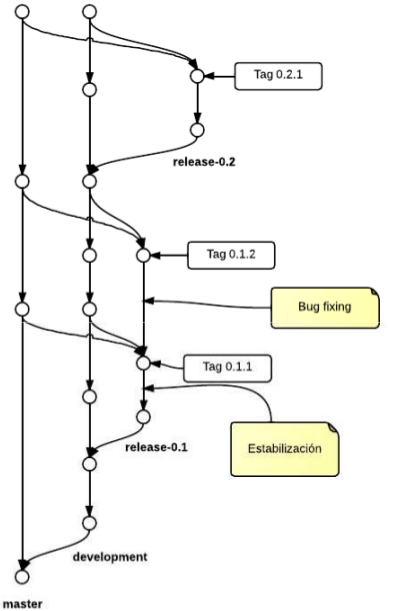
\includegraphics{images/flujo-desarrollo-git-000.png}
\caption{}
\end{figure}

\section{Gestión de repositorios Git con Gerrit}

El primer usuario que se loguea obtiene privilegios de administrador.
Esto es importante si el primero que se loguea lo hace desde el ldap.
Idealmente, debería hacerlo el usuario gerritadmin (ver pasos
previos).\\Gerrit tiene el concepto de grupo, de forma que si asigno
permisos a un grupo para un repositorio, todos los miembros del grupo
adquieren esos permisos.

Los repositorios en jerga Gerrit se denominan proyectos. Pueden crearse
vacíos o con algunas ramas ya preparadas. En nuestro caso todo proyecto
``nacerá'' por simplicidad con dos ramas:

\begin{itemize}
\item
  \texttt{master}
\item
  \texttt{develop}
\end{itemize}
Estos repositorios definen los permisos de acceso en base a referencias
(\texttt{refs/heads/develop}, por ejempo, es la referencia de la rama
\textbf{develop}) que se pueden definir con wildcards como
\texttt{refs/heads/*} (todas las referencias dentro del directorio
\texttt{refs/heads}). Hay diferentes tipos de permisos, más abajo se
explica cómo crear un proyecto con unos permisos razonables para poder
funcionar.

\subsection{Pasos previos}

El primer usuario que accede a Gerrit obtiene privilegios de
administrador. Al instalar la forja, se recomienda crear un usuario
\textbf{``gerritadmin''} y password \textbf{``t0rc0zu310''} y acceder
con este usuario a Gerrit. Este usuario se convertirá en administrador
automáticamente al hacer login. A partir de este momento, este será el
usuario con el que crear los grupos y proyectos (repositorios) en
Gerrit.

Obtener la clave pública del servidor para asignarla al usuario
\textbf{gerritadmin}:

\begin{enumerate}
\item
  \emph{Settings \sout{\textgreater{} SSH Public Keys}\textgreater{}
  Add}
\item
  Copiar la clave del fichero
  \texttt{/opt/ssh-keys/gerritadmin\_rsa.pub}.
\end{enumerate}
Configurar permisos para creación de proyectos:

\begin{enumerate}
\item
  Acceder a \emph{Projects \sout{\textgreater{} List}\textgreater{}
  All-Projects}.
\item
  Seleccionar \emph{Access}:
\item
  \emph{Editar} \sout{\textgreater{} \emph{Add Group}}\textgreater{}
  \emph{Group name} en:
  \begin{itemize}
  \item
    \textbf{refs/} añadir \emph{Push} el grupo \emph{Administrators}.
  \item
    \textbf{refs/meta/config} añadir a \emph{Read} el grupo
    \emph{Administrators}.
  \end{itemize}
\item
  Save Changes.
\end{enumerate}
\subsection{Crear un proyecto}

La Consola de Administración es la encargada de gestionar los
repositorios \texttt{Git} mediante \texttt{gerrit}. Por lo que la
creación de un proyecto Git va asociada a la creación de un nuevo
proyecto en la consola.

\begin{itemize}
\item
  Se ha de elegir un nuevo proyecto asociado a un usuario
  \emph{administrador}.
\item
  Marcar \emph{proyecto con repositorio}.
\item
  Elegir repositorio de tipo \textbf{Git}.
\item
  Grupo de \emph{Usuarios} del proyecto.
\item
  \textbf{Crear proyecto}.
\end{itemize}
\subsection{Comenzar a trabajar en un proyecto}

Asegurarse del mail que se utiliza para la identificación de la autoría
de los commits

\begin{quote}

\end{quote}
\begin{verbatim}
<code class="shell">git config --global user.email "usuario@<dominio-mail.com>"
git config --global user.name "usuario"
git clone ssh://usuario@<dominio.sidelabcode>:29418/<projectname>
cd <projectname>
echo “hello git” > greetings.txt
git add greetings.txt
git commit - "mensaje de commit obligatorio."
</code>
\end{verbatim}
Hasta aquí hemos hecho un commit en el repo local. Para subir este
commit al repo remoto (el que hemos clonado y que se identifica como
origin):

\begin{quote}

\end{quote}
\begin{verbatim}
<code class="shell">git push
</code>
\end{verbatim}
\section{Proceso de desarrollo con Eclipse}

Prerequisitos:

Se recomienda utilizar la versión de Eclipse \textbf{Spring Tools Suite
3.1} de Spring:

\begin{itemize}
\item
  \href{http://www.springsource.org/downloads/sts-ggts}{http://www.springsource.org/downloads/sts-ggts}
\end{itemize}
Se ha de escoger la opción basada en \textbf{Eclipse 3.8.1} ya que
incluye la instalación de las herramientas relacionadas con \texttt{Git}
como es el caso del plugin \href{http://www.eclipse.org/egit/}{Egit}.

Para usar los ejemplos de la línea de comandos se han de instalar los
clientes especificados para cada plataforma que se definieron en el
apartado {[}Clientes git{]}

\subsection{Paso 1 - Generación de claves}

Se han de generar las claves para el acceso al repositorio remoto

\textbf{Ubuntu:}

pre. \$ ssh-keygen -t rsa

\begin{itemize}
\item
  Copiar el contenido del fichero \texttt{\ensuremath{\sim}} en el
  depósito de claves de la cuenta personal de \textbf{Gerrit}.
\end{itemize}
\textbf{Windows:}

pre. Git bash\\ssh-keygen.exe

\begin{itemize}
\item
  Copiar el contenido del fichero
  \texttt{c:/documents and settings/\textless{}usuario\textgreater{}/.ssh/id\_rsa.pub}
  en el depósito de claves de la cuenta personal de \textbf{Gerrit}.
\end{itemize}
\href{https://help.github.com/articles/generating-ssh-keys}{Generating
SSH Keys}

\subsection{Paso 2 - Clonar el repositorio}

El administrador del proyecto ha creado un repositorio en
\textbf{Gerrit} con dos ramas:

\begin{itemize}
\item
  master
\item
  development
\end{itemize}
\subsubsection{Situación del repositorio}

Clonar el repositorio remoto tiene consecuencias:

\begin{itemize}
\item
  El repositorio local guarda localmente información sobre el
  repositorio remoto (llamado por defecto ``origin'')
\item
  Esto permite \emph{subir/bajar} cambios \emph{al/desde} repositorio
  remoto
\item
  Las ramas refs/heads/* del repositorio remoto se almacenan en el
  repositorio local como \texttt{refs/remotes/origin/*}.
\item
  Ver \texttt{.git/config}
\end{itemize}
\subsubsection{Eclipse}

A través de Eclipse se han seguir los siguiente pasos:

\begin{itemize}
\item
  Perspectiva Git repository exploring:
  \texttt{Window -\textgreater{} Open perspective -\textgreater{} Others -\textgreater{} Git Repository Exploring}
\item
  Añadir la \textbf{URI} (la URI es de prueba, se ha de sustituir por
  valores reales) del repositorio y se autocompletan los demás campos:
  \begin{itemize}
  \item
    ssh://patxigortazar\texttt{192.168.33.10:29418/filetransfer
    * Branch selection: dejar ambas seleccionadas
    * Initial branch: seleccionar **development**

    !images/eclipse-clone-repo.png!

    h3. Cliente Git

    Clonar el repositorio remoto a través de la consola:

    pre. \$ git clone ssh://patxigortazar}192.168.33.10:29418/filetransfer
  \end{itemize}
\end{itemize}
\textbf{Git} hace \texttt{checkout del master} por defecto (porque es
donde se encuentra el \emph{HEAD} posicionado en el repositorio remoto).
Se ha de cambiar a la rama \textbf{development} para empezar a
desarrollar:

pre. \$ cd filetransfer\\\$ git checkout development\\Branch development
set up to track remote branch development from origin.\\Switched to a
new branch `development'

\subsection{Paso 3 - crear el proyecto}

\begin{enumerate}
\item
  Se ha de crear un proyecto Java:
  \begin{itemize}
  \item
    \texttt{org.filetransfer}
  \end{itemize}
\item
  Crear un fichero de versión en la raíz
  \begin{itemize}
  \item
    Version.txt \textless{}- 0.1
  \end{itemize}
\item
  Crear un fichero \texttt{SFTPTransfer} en el paquete
  \texttt{org.filetransfer}.
\item
  Añadir el proyecto al repositorio git del proyecto
  \texttt{org.filetransfer}.
  \begin{enumerate}
  \item
    Eclipse:
    \begin{enumerate}
    \item
      \texttt{Team \textgreater{} Share project \textgreater{} Git}
    \item
      \texttt{Repository: filetransfer}
    \item
      Añadir los ficheros para que Eclipse haga tracking de los mismos
    \item
      \texttt{Team \textgreater{} Add to index}
    \end{enumerate}
  \item
    Cliente Git:
    \begin{itemize}
    \item
      \texttt{\$ git status}
    \item
      \texttt{\$ git add \textless{}file\textgreater{}}
    \end{itemize}
  \end{enumerate}
\item
  \textbf{Commit!}
\end{enumerate}
\subsubsection{Commit}

Eclipse:

\begin{enumerate}
\item
  Sobre el proyecto \textgreater{} Team \textgreater{} Commit
\item
  El comentario es obligatorio
\item
  Chequear
  \begin{enumerate}
  \item
    Que el autor es el correcto
  \item
    Que están marcados los ficheros adecuados
  \item
    Que \textbf{no está marcada} la casilla \emph{``Push the changes to
    upstream''}.
  \end{enumerate}
\end{enumerate}
Cliente Git:

pre. git commit

\subsection{Paso 4 - desarrollo de la versión actual}

Añadir algún método más a la clase \texttt{SFTPTransfer} y ejecutar el
comando \texttt{git status}:

pre. \$ git status\\\# On branch develop\\\# Your branch is ahead of
`origin/develop' by 1 commit.\\\#\\\# Changes not staged for commit:\\\#
(use ``git add \ldots{}'' to update what will be committed)\\\# (use
``git checkout --- \ldots{}'' to discard changes in working
directory)\\\#\\\# modified: SFTPTransfer.java\\\#\\no changes added to
commit (use ``git add'' and/or ``git commit -a'')

Hay ficheros no añadidos al staging area por lo que no se hará commit de
ellos.

\begin{figure}[htbp]
\centering
\includegraphics{images/eclipse-git-console-stage.png}
\caption{}
\end{figure}

\subsubsection{git add}

Añadir algún método más a la clase \texttt{SFTPTransfer} y ejecutar el
comando \texttt{git status}:

pre. git status

Hay ficheros no añadidos al staging area no se hará commit de ellos

pre. git add SFTPTransfer.java

Para añadirlos al staging area y que vayan en el próximo commit

pre. \$ git status\\\# On branch develop\\\# Your branch is ahead of
`origin/develop' by 1 commit.\\\#\\\# Changes to be committed:\\\# (use
``git reset HEAD \ldots{}'' to unstage)\\\#\\\# modified:
SFTPTransfer.java\\\#

En Eclipse este proceso se hace automáticamente al hacer
\textbf{commit}.\\En consola se puede forzar con el parámetro
\textbf{-a} al ejecutar:

pre. git commit -a

\subsection{Paso 5 - subir cambios al repositorio remoto (push)}

En este momento el repositorio local se encuentra ``a 2 commits'' del
repositorio remoto.

\begin{figure}[htbp]
\centering
\includegraphics{images/repo-2-commits-ahead.png}
\caption{}
\end{figure}

Subir lo que hay a la rama develop de origin (el repositorio remoto)

\begin{itemize}
\item
  Eclipse:
  \texttt{Sobre el proyecto \textgreater{} Team \textgreater{} Push to upstream}
\item
  Cliente git consola: \texttt{git push origin}
\end{itemize}
\subsection{Paso 6 - estabilización de la versión 0.1}

Se ha de seguir el proceso para unificar los desarrollos del proyecto en
una rama estable y crear el respectivo tag.

\subsubsection{Rama de Versión}

Crear un branch para la versión.

\begin{itemize}
\item
  Eclipse:
  \begin{itemize}
  \item
    Sobre el
    \texttt{proyecto \textgreater{} Team \textgreater{} Switch to \textgreater{} New branch}
    \begin{itemize}
    \item
      From: refs/heads/development
    \item
      Branch name: release--0.1
    \item
      Asegurarse de que checkout new branch está activado
    \end{itemize}
  \end{itemize}
\item
  Cliente git:
  \begin{itemize}
  \item
    \texttt{git checkout -b release-0.1 -{}-track}
  \item
    \texttt{git push -u origin release-0.1}
  \end{itemize}
\end{itemize}
El código del workspace señala ahora la versión
\textbf{release--0.1}.\\* Hacer algún cambio\\* Commit

\subsubsection{Actualizar desarrollo}

\begin{itemize}
\item
  Cambiar en la rama development la \textbf{versión a 0.2}.
\item
  Sobre el
  \texttt{proyecto \textgreater{} Team \textgreater{} Switch to \textgreater{} development}.
\item
  Modificar el fichero \texttt{version.txt}.
\item
  \texttt{Commit}
\item
  \texttt{Push to upstream}
\end{itemize}
\subsubsection{Crear el Tag}

Preparar la RC1 (\emph{Release Candidate 1}).

\begin{itemize}
\item
  Sobre el
  \texttt{proyecto \textgreater{} Team \textgreater{} Switch to \textgreater{} release-0.1}
\item
  Cambiar el nombre de la versión a \textbf{0.1.0-RC1}.
  \begin{itemize}
  \item
    \texttt{Commit}
  \item
    \texttt{Push to upstream}
  \end{itemize}
\end{itemize}
Hacer el tag.

\begin{itemize}
\item
  Eclipse:
  \begin{itemize}
  \item
    \texttt{Team \textgreater{} Advanced \textgreater{} Tag \textgreater{} 0.1.0-RC1}
  \item
    \texttt{Team \textgreater{} Remote \textgreater{} Push... \textgreater{} Next \textgreater{} Add all tags spec}
  \end{itemize}
\item
  Cliente Git:
  \begin{itemize}
  \item
    \texttt{git tag -a 0.1.0-RC1 -m 'Release 0.1.0-RC1`}
  \item
    \texttt{git push origin 0.1.0-RC1}
  \end{itemize}
\end{itemize}
Ejecutar el ciclo de \textbf{Build/test/deploy\ldots{}}

\subsection{Paso 7 - publicar la versión 0.1.0}

Si el desarrollo, las pruebas y los despliegues son correctos en la rama
\textbf{RCx}:

* Cambiar el nombre de la versión a \textbf{0.1.0}.\\\textbf{*
Commit\\}* Push to upstream\\Hacer el tag.\\* Eclipse:\\\textbf{*
\texttt{Team \textgreater{} Advanced \textgreater{} Tag \textgreater{} 0.1.0}\\}*
\texttt{Team \textgreater{} Remote \textgreater{} Push... \textgreater{} Next \textgreater{} Add all tags spec}\\\textbf{*
Marcar \emph{``Save in origin''} para añadirlo a la configuración del
repositorio\\} Cliente git:\\\textbf{*
\texttt{git tag -a 0.1.0 -m 'Version 0.1.0`}\\}*
\texttt{git push origin 0.1.0}

Volver a ejecutar el ciclo de \textbf{Build/test/deploy\ldots{}}

\subsection{Paso 8 - integrar los cambios en development}

Se han de integrar los cambios de la nueva version en la rama de
desarrollo\\ \textbf{development}. Esta acción se conoce como
\textbf{merge}.

Eclipse\\*
\texttt{Team \textgreater{} Switch to \textgreater{} deve lopment}\\*
\texttt{Team \textgreater{} Merge \textgreater{} Tags \textgreater{} 0.1.0}

\textbf{Conflictos en el fichero version.txt\includegraphics{}}

\begin{itemize}
\item
  Abrir el fichero version.txt
\item
  Dejar la versión 0.2 y quitar todo lo demás
\end{itemize}
Para indicar que los conflictos han sido resueltos:

\begin{itemize}
\item
  Eclipse: Sobre el fichero \textgreater{} Team \textgreater{} Add to
  index
\item
  Cliente git: \texttt{git add \textless{}fichero\textgreater{}}
\item
  Commit
\end{itemize}
\subsubsection{Si todo va mal en un merge}

Se ha de hacer un \textbf{Reset}.

Así se actualiza el índice (base de datos de git), el HEAD y la carpeta
de trabajo con la versión que le digamos

\begin{itemize}
\item
  Eclipse:
  \texttt{Team \textgreater{} Reset... \textgreater{} elegir un branch \textgreater{} Marcar HARD}
\item
  Cliente git:
  \texttt{git reset -{}-hard \textless{}branch\textgreater{}}
\end{itemize}
\subsection{Paso 9 - bug fixing}

El proceso para arreglar \textbf{bugs} y \textbf{hotfixes} para
integrarlo en el desarrollo mediante ramas.

\begin{itemize}
\item
  Eclipse:
  \texttt{Team \textgreater{} Switch to \textgreater{} release-0.1}
\item
  Cliente git: \texttt{\$ git checkout development}
  \begin{itemize}
  \item
    Cambiar la versión a 0.1.1-RC1
  \item
    Arreglar el bug
  \item
    Mismo proceso que con la 0.1.0-RCx
  \item
    Eclipse:
    \texttt{Team \textgreater{} Merge \textgreater{} Tags \textgreater{} 0.1.1-RC1}
  \end{itemize}
\end{itemize}
Volver a repetir el cicloe de \textbf{Release} y \textbf{Tag}:

\begin{itemize}
\item
  Cuando se considere suficientemente estable: release
\item
  Cambiar versión a 0.1.1
\item
  Tag 0.1.1
\item
  Mezclar con development
\item
  Mezclar con master
\end{itemize}
\subsection{Paso 10 - obtener cambios del repositorio remoto (pull)}

Representar el escenario de programación en pareja con dos roles y las
distintas acciones sobre los ficheros.

\begin{itemize}
\item
  Rol A
\item
  Rol B
\end{itemize}
\# \texttt{A} modifica el fichero java:\\* Hacer \texttt{commit} de los
cambios.\\* \texttt{Push to upstream}\\\# \texttt{B} obtiene los
cambios:\\* Sobre el
\texttt{proyecto \textgreater{} Team \textgreater{} Fetch from upstream}
para obtener el índice de cambios\\* Sobre el
\texttt{proyecto \textgreater{} Team \textgreater{} Pull}

\subsubsection{Resolución de conflictos}

¿Qué pasa si otro desarrollador subió cambios que entran en conflicto
con los míos?

\begin{itemize}
\item
  A modifica el constructor
\item
  B modifica el constructor de otra manera diferente
\item
  A y B hacen push del repositorio
\end{itemize}
Obtener los cambios:

\begin{itemize}
\item
  \texttt{Team \textgreater{} Fetch from upstream}
\item
  \texttt{Team \textgreater{} Pull}
\end{itemize}
Los cambios se mezclan y git marca los conflictos para resolver.\\Se han
de corregir \emph{manualmente} los conflictos y añadir al
\emph{upstream}.

\begin{itemize}
\item
  \texttt{git add \textless{}fichero\textgreater{}}
\item
  \texttt{git commit}
\item
  \texttt{git push origin \textless{}rama\textgreater{}}
\end{itemize}
\subsection{Comandos útiles}

Git ofrece una lista de acciones relacionadas con el repositorio
distribuido para el desarrollo basado en ramas ya que hay mucha
información y nos ofrece una forma de gestionarla.

\subsubsection{Commit Log}

El histórico de \emph{commits} en git se conoce como log. Debido a que
los comentarios asociados a los commits son \textbf{obligatorios}
tenemos un historial bastante potente.

\begin{itemize}
\item
  Información de los commits: \texttt{git log}
\item
  Información de lo que ha cambiado en los últimos dos commits:
  \texttt{git log -p -2}
\item
  Información de los commits enlazando la estrucutra de padres e hijos y
  ramas \texttt{git log -{}-graph}
\end{itemize}
\subsubsection{Deshacer acciones}

Deshacer commits en git se podría comparar \texttt{subversion revert}
pero funcional.\\Nos permite añadir nuevos ficheros, actualizar los
comentarios, eliminar ficheros que no deberían entrar en ese commit, es
decir rehacer el \emph{último commit}.

\begin{itemize}
\item
  \texttt{git commit -{}-amend}
\end{itemize}
\section{Integración continua}

\subsection{Cómo vamos a hacer CI}

\begin{figure}[htbp]
\centering
\includegraphics{images/jenkins_logo.png}
\caption{}
\end{figure}

Usaremos un servidor de CI: \href{http://jenkins-ci.org/}{Jenkins}
Jenkins realizará determinadas tareas de forma automática:\\* Tags\\*
Construir las versiones vivas

También proveerá tareas para ser ejecutadas manualmente\\* Branches de
releases\\* Desplegar una versión específica con un clic

Las versiones vivas vivirán en su propia máquina virtual

\begin{figure}[htbp]
\centering
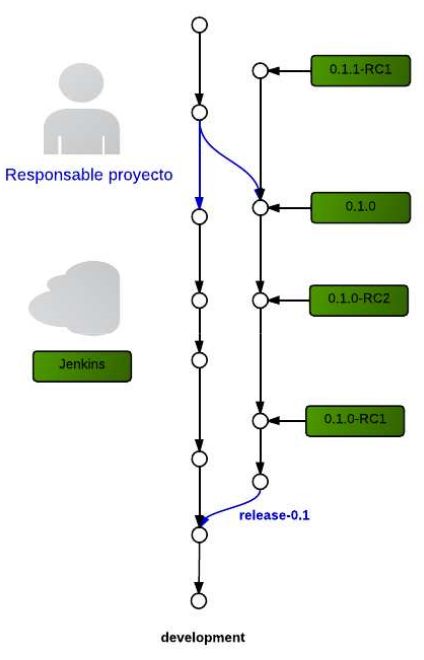
\includegraphics{images/jenkins-git.png}
\caption{}
\end{figure}

\subsubsection{Objetivos}

Se mantendrán diferentes versiones vivas a la vez para cumplir unos
objetivos: \\* Asegurar la calidad\\* Hacer el despliegue ágil\\*
Minimizar el riesgo

\begin{quote}
``Release early, release often''

\end{quote}
\subsubsection{Proceso}

El repositorio remoto debería contener versiones más o menos estables

\includegraphics{images/integracion-co-test.png}\\\includegraphics{images/integracion-tag-deploy.png}\\\includegraphics{images/despliegue-produccion.png}

\textbf{Develop}\\* Pueden fallar algunos tests, no es problema.\\* La
versión del último commit se despliega en \emph{``local''}

\textbf{Release-X}\\* Los tests deberían pasar, eventualmente se podrían
desactivar.\\* La versión del \emph{último commit} se despliega en
\emph{``local''}.

\textbf{Nightly builds}\\* Construcciones que comprueban la
\emph{``salud''} del proyecto.\\* Se hacen sobre los branches
\emph{development} y \emph{release-X} (siendo X la versión más
reciente).\\* Se ejecutan los tests.\\* Se despliegan dos versiones por
cada rama:\\\textbf{* \texttt{Limpia}: una bbdd nueva.\\}*
\texttt{Migración}: con actualización de bbdd ya existente sobre la bbdd
que ya hubiera para ese despliegue.

\textbf{Preproducción}\\* Las versiones que van a preproducción son
aquellas de las que se ha hecho \texttt{tag}.\\* Pasan los tests.\\* El
entorno de pre puede estar en \emph{local} o en \emph{Amazon}.\\* Se
despliegan dos versiones.\\\textbf{* \texttt{Limpia}.\\}*
\texttt{Migración}.

\textbf{Producción}\\* Las versiones que van a producción son aquellas
de las que se ha hecho \texttt{tag}.\\* Pasan los tests\\* El despliegue
se realiza en \emph{Amazon}.\\* Se despliegan dos versiones:\\\textbf{*
\texttt{Limpia}.\\}* \texttt{Migración}.

\begin{figure}[htbp]
\centering
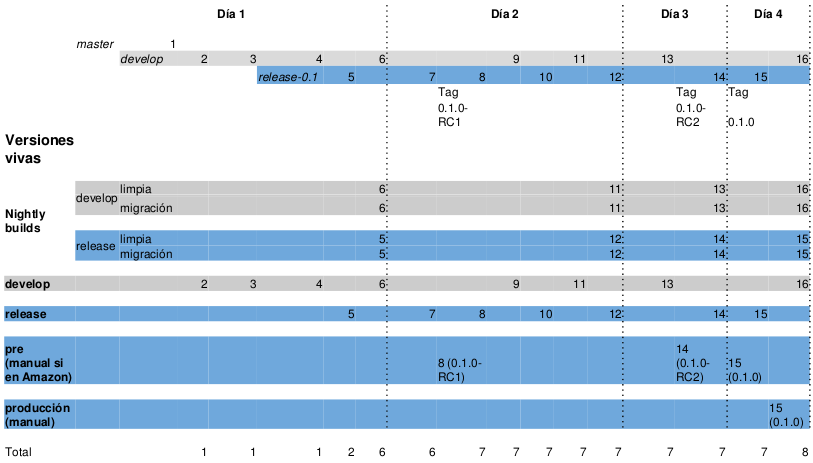
\includegraphics{images/diagrama-integracion-continua.png}
\caption{}
\end{figure}

\subsection{Configuración de Jenkins}

Configurar \emph{Jenkins} para acceder a múltiples repositorios git.
Para esto se han de tener en cuenta los siguientes requerimientos:

\begin{itemize}
\item
  \emph{Jenkins} construye diferentes proyectos en donde en proyecto
  puede tener su propio repositorio git.
\item
  \emph{Jenkins} debe tener permisos de lectura o lectura/escritura a
  todos los repositorios de aquellos proyectos que vaya a construir.
\item
  Por defecto \emph{Jenkins} usa la clave del usuario en
  \texttt{\ensuremath{\sim}} para autenticarse
\item
  ¿Con qué usuario se ejecuta Jenkins? con el usuario \textbf{tomcat}.
\end{itemize}
\subsubsection{Opciones}

\textbf{Opción I}: Un usuario \texttt{jenkinsci} con acceso de
\emph{lectura/escritura} a \textbf{todos} los repositorios.\\*
\textbf{Pros}:\\\textbf{* \emph{Simplicidad}: sólo hay que gestionar un
usuario.\\}* Una \textbf{única} clave ssh
\texttt{/home/tomcat/.ssh/id\_rsa.pub}.\\* \textbf{Contras}:\\\textbf{*
Un usuario para dominarlos a todos.\\}* Cualquier error en un job para
el proyecto \emph{X} puede afectar a los repositorios del proyecto
\emph{Y}.\\\textbf{Opción II}: Un usuario \texttt{jenkinsci} con acceso
de \emph{lectura/escritura} a todos los repositorios y otro
\texttt{jenkinsci\_read} con acceso sólo de lectura\\*
\textbf{Pros}:\\\textbf{* Sólo hay que gestionar \emph{dos usuarios}:
basta con asociarlos a}\textbf{todos}* los proyectos.\\*
\textbf{Contras}:\\\textbf{* Seguimos teniendo un usuario para
dominarlos a todo: jenkinsci\\}* Cualquier error en un job para el
proyecto \emph{X} puede afectar a los repositorios del proyecto
\emph{Y}.\\\textbf{* Hay que gestionar dos claves ssh\ldots{} no es
trivial\\}\textbf{Opción III}\textbf{: Un}\textbf{usuario por proyecto}*
para integración continua.\\* \textbf{Pros}:\\\textbf{* El usuario de ci
de un proyecto no tiene acceso a los repos de otro proyecto.\\}
\textbf{Contras}:\\** Hay que gestionar múltiples \texttt{claves ssh}.

\textbf{Utilizaremos la Opción III}

\subsubsection{Configurar Opción III}

Configurar \emph{Jenkins} para acceso a \emph{múltiples repositorios
git} siguiendo los siguientes pasos:\\* Crear los usuarios necesarios en
la forja.\\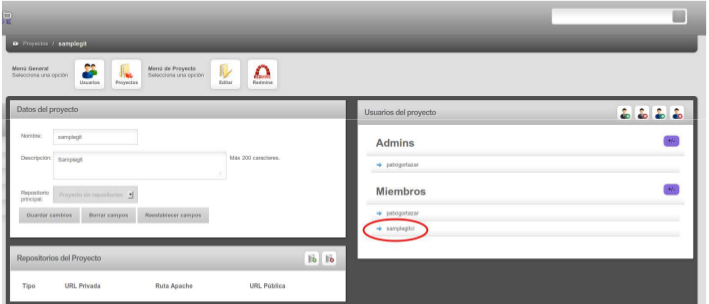
\includegraphics{images/gestion-jenkins-usuarios-000.png}\\*
Generar un par de claves pública/privada con \texttt{ssh-keygen} para
cada usuario en diferentes ficheros.\\* Acceder a Gerrit con cada
usuario
creado.\\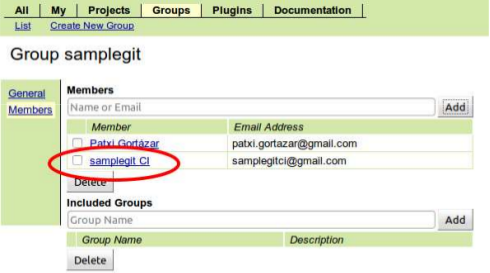
\includegraphics{images/gestion-jenkins-usuarios-001.png}\\*
Añadir la clave pública para este usuario.\\* Copiar las claves a la
máquina de Jenkins.\\** Carpeta \texttt{/opt/ssh-keys}.

\begin{quote}

\end{quote}
\begin{verbatim}
<code class="shell">$ cd /opt/ssh-keys
$ ll
total 24
drwxr-xr-x  2 tomcat tomcat 4096 Jan  4 09:46 ./
drwxr-xr-x 14 root   root   4096 Jan  4 09:42 ../
- rw-------  1 tomcat tomcat 1679 Jan  4 09:46 filetransferci_rsa
- rw-r--r--  1 tomcat tomcat  398 Jan  4 09:46 filetransferci_rsa.pub
- rw-------  1 tomcat tomcat 1679 Jan  4 09:44 samplegitci_rsa
- rw-r--r--  1 tomcat tomcat  396 Jan  4 09:44 samplegitci_rsa.pub
</code>
\end{verbatim}
\begin{itemize}
\item
  Configurar SSH para que utilice la clave correcta en cada caso.
  \begin{itemize}
  \item
    Crear el fichero \texttt{/home/tomcat/.ssh/config}.
  \end{itemize}
\end{itemize}
\begin{quote}

\end{quote}
\begin{verbatim}
<code class="shell">$ cd /home/tomcat/.ssh
$ cat config
Host samplegit.patxi.sidelab.es
    HostName patxi.sidelab.es
    User samplegitci
    IdentityFile /opt/ssh-keys/samplegitci_rsa
Host filetransfer.patxi.sidelab.es
    HostName patxi.sidelab.es
    User filetransferci
    IdentityFile /opt/ssh-keys/filetransferci_rsa
</code>
\end{verbatim}
\subsection{Configuración de builds}

Los builds de \emph{Jenkins} funcionan a través de la configuración de
\textbf{jobs}. Por lo que vamos a definir los jobs necesarios para el
proceso de integración continua.

Se dividen en tres grupos:

\begin{itemize}
\item
  Jobs de \textbf{integración} (read only).
  \begin{itemize}
  \item
    Descargan el código (checkout).
  \item
    Construyen.
  \item
    Pasan tests.
  \item
    Despliegan la versión construida en ``local''.
  \end{itemize}
\item
  Jobs de \textbf{release} (read/write).
  \begin{itemize}
  \item
    Realizan los pasos anteriores y además.
  \item
    Tag si los tests pasaron.
  \item
    Push del tag al repositorio remoto.
  \end{itemize}
\item
  Jobs de \textbf{despliegue} (read only).
  \begin{itemize}
  \item
    Descargan el binario del repositorio de binarios
  \item
    Desplegar
  \end{itemize}
\end{itemize}
\subsubsection{Job de integración}

* Crear un \textbf{job} \emph{\#Maven}.\\* Configurar el repositorio
git\\\textbf{*
\texttt{ssh://filetransferci}filetransferci.code.tscompany.es/filetransfer@\\}*
Ssh leerá el fichero config y utilizará el fichero de claves
correspondiente el host \texttt{filetransferci.code.tscompany.es}.\\*
Añadir las ramas a construir (añadir nuevas ramas con el botón
``Add'')\\\textbf{* \texttt{development}\\}* \texttt{release-0.1.1}\\*
Añadir el \texttt{user.email} y \texttt{user.name} que usará
\emph{Jenkins}.\\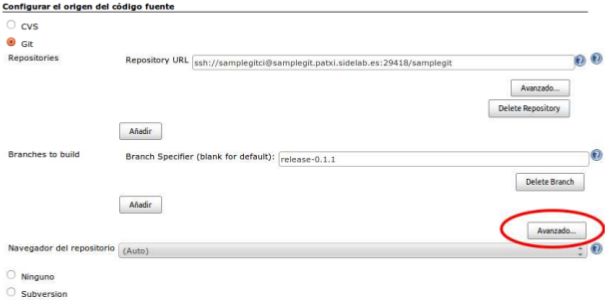
\includegraphics{images/jenkins-job-integracion.png}\\*
Los resultados del build se pueden comprobar en:\\\textbf{*
\texttt{/opt/jenkins/jobs/filetransfer/workspace}\\}* Si es un proyecto
\emph{Maven}, dentro del proyecto en la carpeta target estará el
artefacto generado.\\\textbf{* También se puede acceder vía
web.\\}\textbf{* Y descargar el workspace como un}zip\textbf{.\\}* Los
\textbf{tests} están en la carpeta \texttt{surfire-reports} del proyecto
\emph{Maven}.\\\textbf{* También pueden consultarse}vía web* accediendo
al build y seleccionando \emph{``Resultado de los
tests''}.\\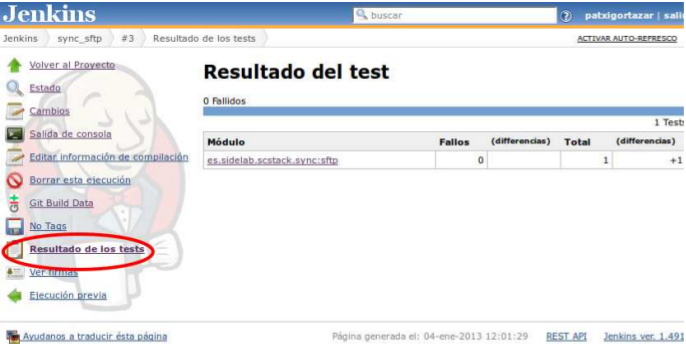
\includegraphics{images/jenkins-job-resultados.png}

\subsection{Maven}

\emph{Jenkins} permite construir proyectos
\href{http://maven.apache.org/}{Maven}.

En determinadas ocasiones los proyectos requieren configuraciones
específicas. La información sensible suele ir en el fichero
\texttt{settings.xml} en el \texttt{home} del usuario en su máquina de
desarrollo-

\begin{itemize}
\item
  Info de \textbf{autenticación para Archiva}.
\item
  \textbf{Profiles}
\end{itemize}
En Jenkins esto se puede gestionar con el plugin \emph{``Config File
Provider Plugin''}.

\begin{figure}[htbp]
\centering
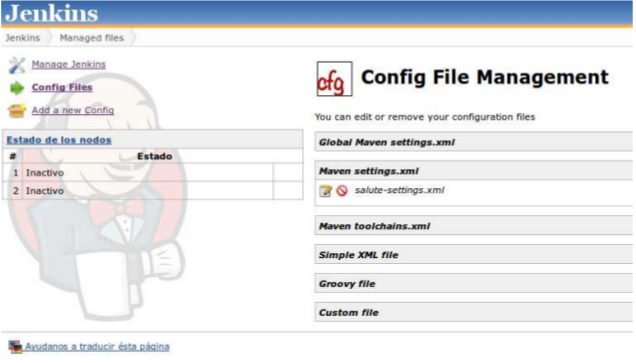
\includegraphics{images/jenkins-config-file-management.png}
\caption{}
\end{figure}

Podemos añadir cualquiera de los ficheros creados con \emph{Config File
Management} en un \textbf{job}.

\begin{figure}[htbp]
\centering
\includegraphics{images/jenkisn-config-file-management-settings.png}
\caption{}
\end{figure}

Para los deploys, si el certificado es autofirmado es \textbf{necesario}
generar un \textbf{truststore} a partir del certificado generado por el
servidor:

\begin{itemize}
\item
  \href{http://www.liferay.com/web/neil.griffin/blog/-/blogs/fixing-suncertpathbuilderexception-caused-by-maven-downloading-from-self-signed-repository}{http://www.liferay.com/web/neil.griffin/blog/-/blogs/fixing-suncertpathbuilderexception-caused-by-maven-downloading-from-self-signed-repository}
\end{itemize}
Este truststore debe incluirse en todos los \texttt{jdk} que utilice
\emph{Jenkins} en la ruta indicada en el enlace anterior

